\documentclass{article}\usepackage{graphicx, color}
%% maxwidth is the original width if it is less than linewidth
%% otherwise use linewidth (to make sure the graphics do not exceed the margin)
\makeatletter
\def\maxwidth{ %
  \ifdim\Gin@nat@width>\linewidth
    \linewidth
  \else
    \Gin@nat@width
  \fi
}
\makeatother

\IfFileExists{upquote.sty}{\usepackage{upquote}}{}
\definecolor{fgcolor}{rgb}{0.2, 0.2, 0.2}
\newcommand{\hlnumber}[1]{\textcolor[rgb]{0,0,0}{#1}}%
\newcommand{\hlfunctioncall}[1]{\textcolor[rgb]{0.501960784313725,0,0.329411764705882}{\textbf{#1}}}%
\newcommand{\hlstring}[1]{\textcolor[rgb]{0.6,0.6,1}{#1}}%
\newcommand{\hlkeyword}[1]{\textcolor[rgb]{0,0,0}{\textbf{#1}}}%
\newcommand{\hlargument}[1]{\textcolor[rgb]{0.690196078431373,0.250980392156863,0.0196078431372549}{#1}}%
\newcommand{\hlcomment}[1]{\textcolor[rgb]{0.180392156862745,0.6,0.341176470588235}{#1}}%
\newcommand{\hlroxygencomment}[1]{\textcolor[rgb]{0.43921568627451,0.47843137254902,0.701960784313725}{#1}}%
\newcommand{\hlformalargs}[1]{\textcolor[rgb]{0.690196078431373,0.250980392156863,0.0196078431372549}{#1}}%
\newcommand{\hleqformalargs}[1]{\textcolor[rgb]{0.690196078431373,0.250980392156863,0.0196078431372549}{#1}}%
\newcommand{\hlassignement}[1]{\textcolor[rgb]{0,0,0}{\textbf{#1}}}%
\newcommand{\hlpackage}[1]{\textcolor[rgb]{0.588235294117647,0.709803921568627,0.145098039215686}{#1}}%
\newcommand{\hlslot}[1]{\textit{#1}}%
\newcommand{\hlsymbol}[1]{\textcolor[rgb]{0,0,0}{#1}}%
\newcommand{\hlprompt}[1]{\textcolor[rgb]{0.2,0.2,0.2}{#1}}%

\usepackage{framed}
\makeatletter
\newenvironment{kframe}{%
 \def\at@end@of@kframe{}%
 \ifinner\ifhmode%
  \def\at@end@of@kframe{\end{minipage}}%
  \begin{minipage}{\columnwidth}%
 \fi\fi%
 \def\FrameCommand##1{\hskip\@totalleftmargin \hskip-\fboxsep
 \colorbox{shadecolor}{##1}\hskip-\fboxsep
     % There is no \\@totalrightmargin, so:
     \hskip-\linewidth \hskip-\@totalleftmargin \hskip\columnwidth}%
 \MakeFramed {\advance\hsize-\width
   \@totalleftmargin\z@ \linewidth\hsize
   \@setminipage}}%
 {\par\unskip\endMakeFramed%
 \at@end@of@kframe}
\makeatother

\definecolor{shadecolor}{rgb}{.97, .97, .97}
\definecolor{messagecolor}{rgb}{0, 0, 0}
\definecolor{warningcolor}{rgb}{1, 0, 1}
\definecolor{errorcolor}{rgb}{1, 0, 0}
\newenvironment{knitrout}{}{} % an empty environment to be redefined in TeX

\usepackage{alltt}
\usepackage[sc]{mathpazo}
\usepackage{geometry}
\geometry{verbose,tmargin=2.5cm,bmargin=2.5cm,lmargin=2.5cm,rmargin=2.5cm}
\setcounter{secnumdepth}{2}
\setcounter{tocdepth}{2}
\usepackage{url}
\usepackage[unicode=true,pdfusetitle, bookmarks=true,bookmarksnumbered=true,bookmarksopen=true,bookmarksopenlevel=2, breaklinks=false,pdfborder={0 0 1},backref=false,colorlinks=false] {hyperref}
\hypersetup{ pdfstartview={XYZ null null 1}}
\usepackage{breakurl}
\parindent = 0pt

\usepackage{amsmath}
\usepackage{framed, color}
\definecolor{shadecolor}{RGB}{211, 211, 211}

\title{Mike Lederle\\lederle@neo.tamu.edu\\STAT 607 --- HW 4}

\begin{document}


\maketitle
\section*{Exercise 4.3}
\subsection*{Exercise 4.3 (a)}
\begin{knitrout}
\definecolor{shadecolor}{rgb}{0.969, 0.969, 0.969}\color{fgcolor}\begin{kframe}
\begin{alltt}
diameter <- \hlfunctioncall{c}(12, 11.4, 7.9, 9, 10.5, 7.9, 7.3, 10.2, 11.7, 11.3, 5.7, 8, 10.3, 12, 9.2, 8.5, 
    7, 10.7, 9.3, 8.2)
age <- \hlfunctioncall{c}(125, 119, 83, 85, 99, 117, 69, 133, 154, 168, 61, 80, 114, 147, 122, 106, 82, 88, 
    97, 99)
trees <- \hlfunctioncall{data.frame}(diameter, age)
\hlfunctioncall{qplot}(diameter, age, trees)
\end{alltt}
\end{kframe}

{\centering 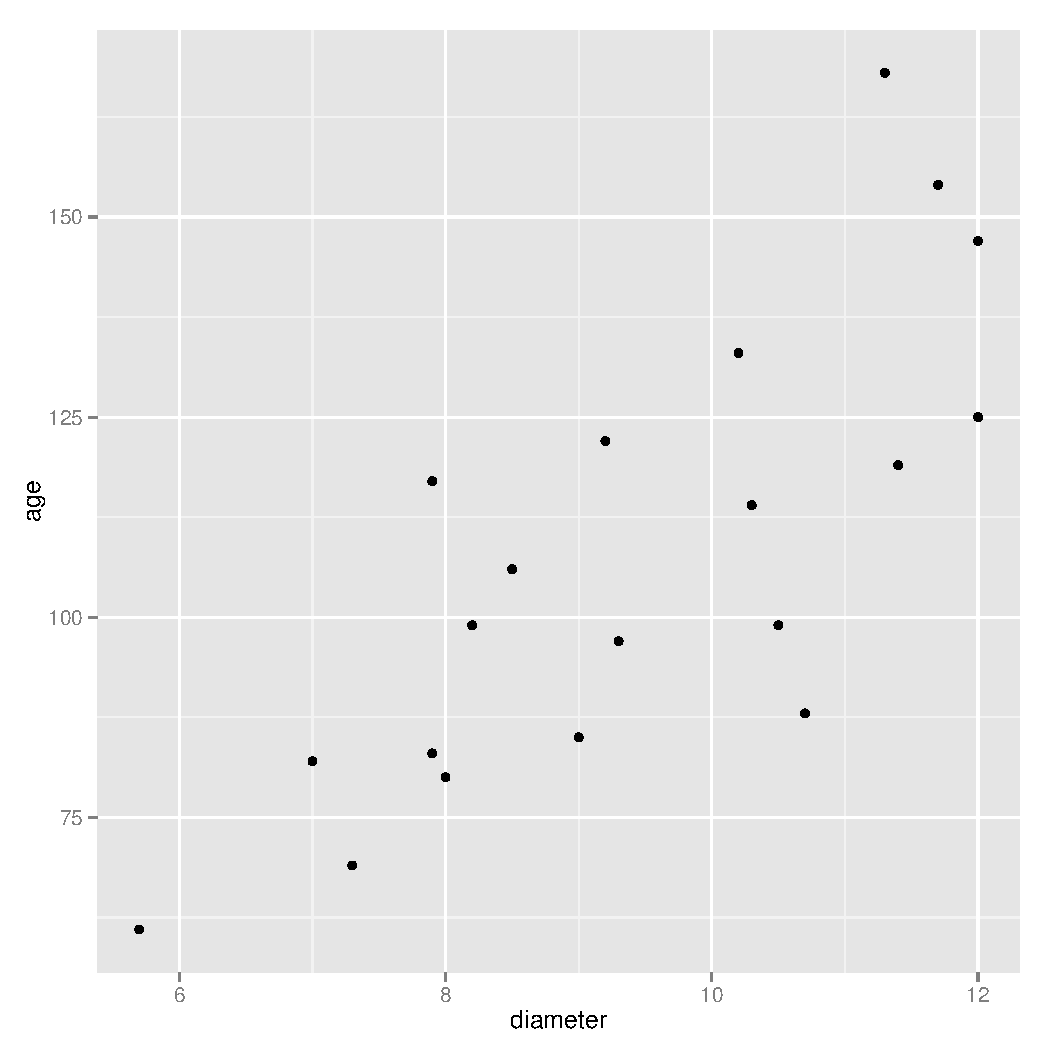
\includegraphics[width=.45\textwidth]{figure/unnamed-chunk-1} 

}


\end{knitrout}


\subsection*{Exercise 4.3 (b)}
\begin{knitrout}
\definecolor{shadecolor}{rgb}{0.969, 0.969, 0.969}\color{fgcolor}\begin{kframe}
\begin{alltt}
x.bar.U <- 10.3
N <- 1132
(n <- \hlfunctioncall{nrow}(trees))
\end{alltt}
\begin{verbatim}
## [1] 20
\end{verbatim}
\begin{alltt}
(x.bar <- \hlfunctioncall{mean}(diameter))
\end{alltt}
\begin{verbatim}
## [1] 9.405
\end{verbatim}
\begin{alltt}
(y.bar <- \hlfunctioncall{mean}(age))
\end{alltt}
\begin{verbatim}
## [1] 107.4
\end{verbatim}
\begin{alltt}
(B.hat <- y.bar/x.bar)
\end{alltt}
\begin{verbatim}
## [1] 11.42
\end{verbatim}
\begin{alltt}
y.bar.hat.ratio <- B.hat * x.bar.U
\hlfunctioncall{paste}(\hlstring{"ESTIMATOR OF POP MEAN VIA RATIO ===="}, y.bar.hat.ratio)
\end{alltt}
\begin{verbatim}
## [1] "ESTIMATOR OF POP MEAN VIA RATIO ==== 117.620414673046"
\end{verbatim}
\begin{alltt}
(fpc <- 1 - n/N)
\end{alltt}
\begin{verbatim}
## [1] 0.9823
\end{verbatim}
\begin{alltt}
(term2 <- (x.bar.U/x.bar)^2)
\end{alltt}
\begin{verbatim}
## [1] 1.199
\end{verbatim}
\begin{alltt}
.resid <- \hlfunctioncall{function}(x, y) \{
    y.bar <- \hlfunctioncall{mean}(y)
    x.bar <- \hlfunctioncall{mean}(x)
    y - y.bar/x.bar * x
\}
variance.resid <- \hlfunctioncall{function}(r) \{
    \hlfunctioncall{sum}(r^2)/(\hlfunctioncall{length}(r) - 1)
\}
(term3 <- \hlfunctioncall{variance.resid}(\hlfunctioncall{.resid}(diameter, age))/n)
\end{alltt}
\begin{verbatim}
## [1] 16.1
\end{verbatim}
\begin{alltt}
SE.y.bar.hat.ratio <- \hlfunctioncall{sqrt}(fpc * term2 * term3)
\hlfunctioncall{paste}(\hlstring{"STD ERR OF POP MEAN USING RATIO ===="}, SE.y.bar.hat.ratio)
\end{alltt}
\begin{verbatim}
## [1] "STD ERR OF POP MEAN USING RATIO ==== 4.35487189729141"
\end{verbatim}
\end{kframe}
\end{knitrout}


\subsection*{Exercise 4.3 (c)}
\begin{knitrout}
\definecolor{shadecolor}{rgb}{0.969, 0.969, 0.969}\color{fgcolor}\begin{kframe}
\begin{alltt}
simple.reg <- \hlfunctioncall{function}(x, y) \{
    B.1.hat <- \hlfunctioncall{cor}(x, y) * \hlfunctioncall{sd}(y)/\hlfunctioncall{sd}(x)
    B.0.hat <- \hlfunctioncall{mean}(y) - B.1.hat * \hlfunctioncall{mean}(x)
    \hlfunctioncall{list}(B.0.hat, B.1.hat)
\}
(trees.coef <- \hlfunctioncall{unlist}(\hlfunctioncall{simple.reg}(diameter, age)))
\end{alltt}
\begin{verbatim}
## [1] -7.808 12.250
\end{verbatim}
\begin{alltt}
y.bar.hat.reg <- trees.coef[1] + trees.coef[2] * x.bar.U
\hlfunctioncall{paste}(\hlstring{"ESTIMATOR OF POP MEAN VIA REGRESSION ===="}, y.bar.hat.reg)
\end{alltt}
\begin{verbatim}
## [1] "ESTIMATOR OF POP MEAN VIA REGRESSION ==== 118.36344896498"
\end{verbatim}
\begin{alltt}
se.reg <- \hlfunctioncall{function}(x, y, N) \{
    fpc <- 1 - \hlfunctioncall{length}(x)/N
    \hlfunctioncall{sqrt}(fpc * 1/n * \hlfunctioncall{var}(y) * (1 - \hlfunctioncall{cor}(x, y)^2))
\}
\hlfunctioncall{paste}(\hlstring{"STD ERR OF POP MEAN USING REGRESSION ===="}, \hlfunctioncall{se.reg}(diameter, age, N))
\end{alltt}
\begin{verbatim}
## [1] "STD ERR OF POP MEAN USING REGRESSION ==== 3.96220011630061"
\end{verbatim}
\end{kframe}
\end{knitrout}


\subsection*{Exercise 4.3 (d)}
\begin{knitrout}
\definecolor{shadecolor}{rgb}{0.969, 0.969, 0.969}\color{fgcolor}\begin{kframe}
\begin{alltt}
p <- \hlfunctioncall{qplot}(diameter, age, trees)
p + \hlfunctioncall{geom_abline}(intercept = 0, slope = B.hat) + \hlfunctioncall{geom_abline}(intercept = trees.coef[1], slope = trees.coef[2], 
    color = \hlstring{"red"}) + \hlfunctioncall{geom_hline}(yintercept = y.bar.hat.ratio) + \hlfunctioncall{geom_hline}(yintercept = y.bar.hat.reg, 
    color = \hlstring{"red"})
\end{alltt}
\end{kframe}

{\centering 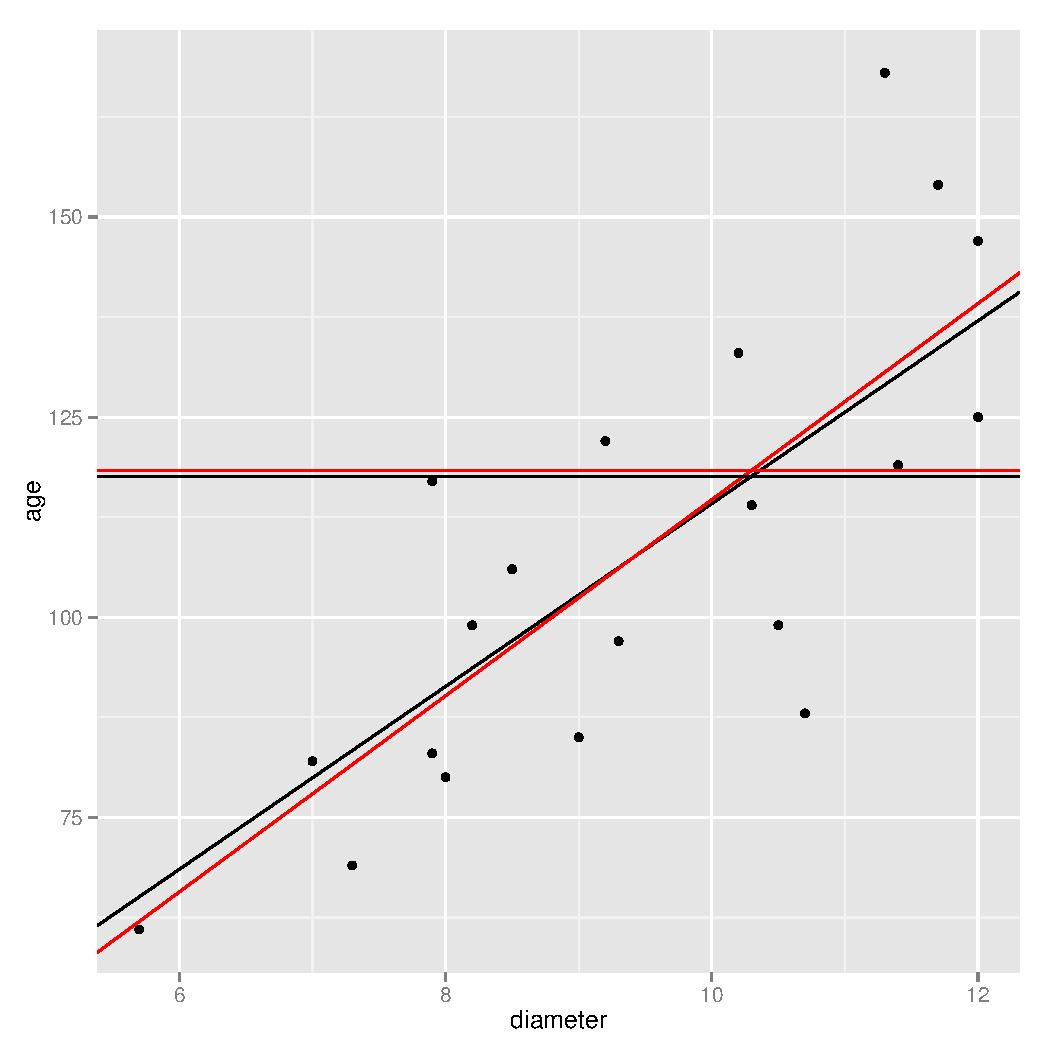
\includegraphics[width=.85\textwidth]{figure/unnamed-chunk-4} 

}


\end{knitrout}

Seem pretty close to me.  Regression estimate has lower SE.
\vfil
\newpage
\section*{Exercise 4.8}
\subsection*{Exercise 4.8 (a)}
\begin{knitrout}
\definecolor{shadecolor}{rgb}{0.969, 0.969, 0.969}\color{fgcolor}\begin{kframe}
\begin{alltt}
agsrs <- \hlfunctioncall{read.csv}(\hlstring{"~/Courses/STAT 607/STAT-607/data/Dataset/agsrs.csv"})
\hlfunctioncall{qplot}(farms87, data = agsrs)
\end{alltt}


{\ttfamily\noindent\itshape\textcolor{messagecolor}{\#\# stat\_bin: binwidth defaulted to range/30. Use 'binwidth = x' to adjust this.}}\begin{alltt}
\hlfunctioncall{qplot}(farms87, farms92, data = agsrs)
\end{alltt}
\end{kframe}

{\centering 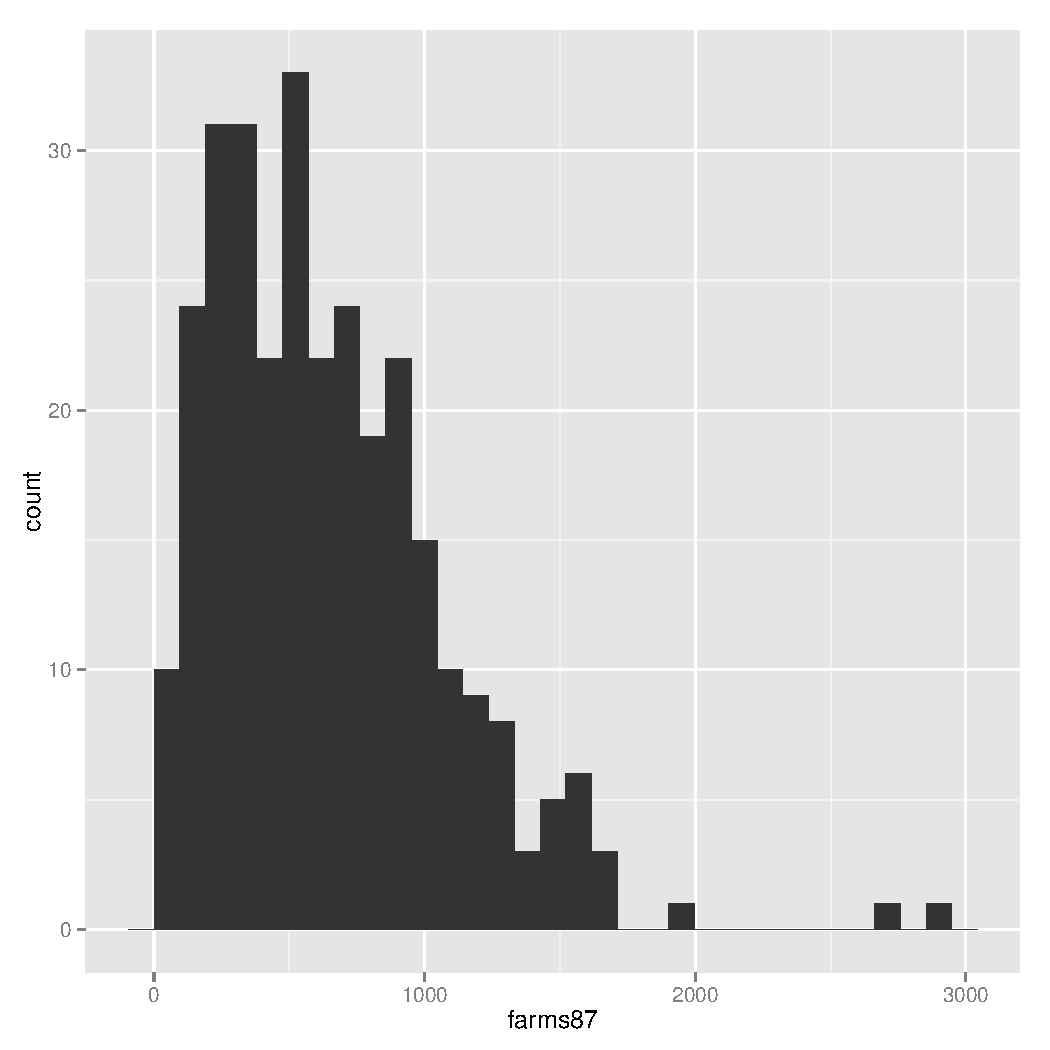
\includegraphics[width=.45\textwidth]{figure/unnamed-chunk-51} 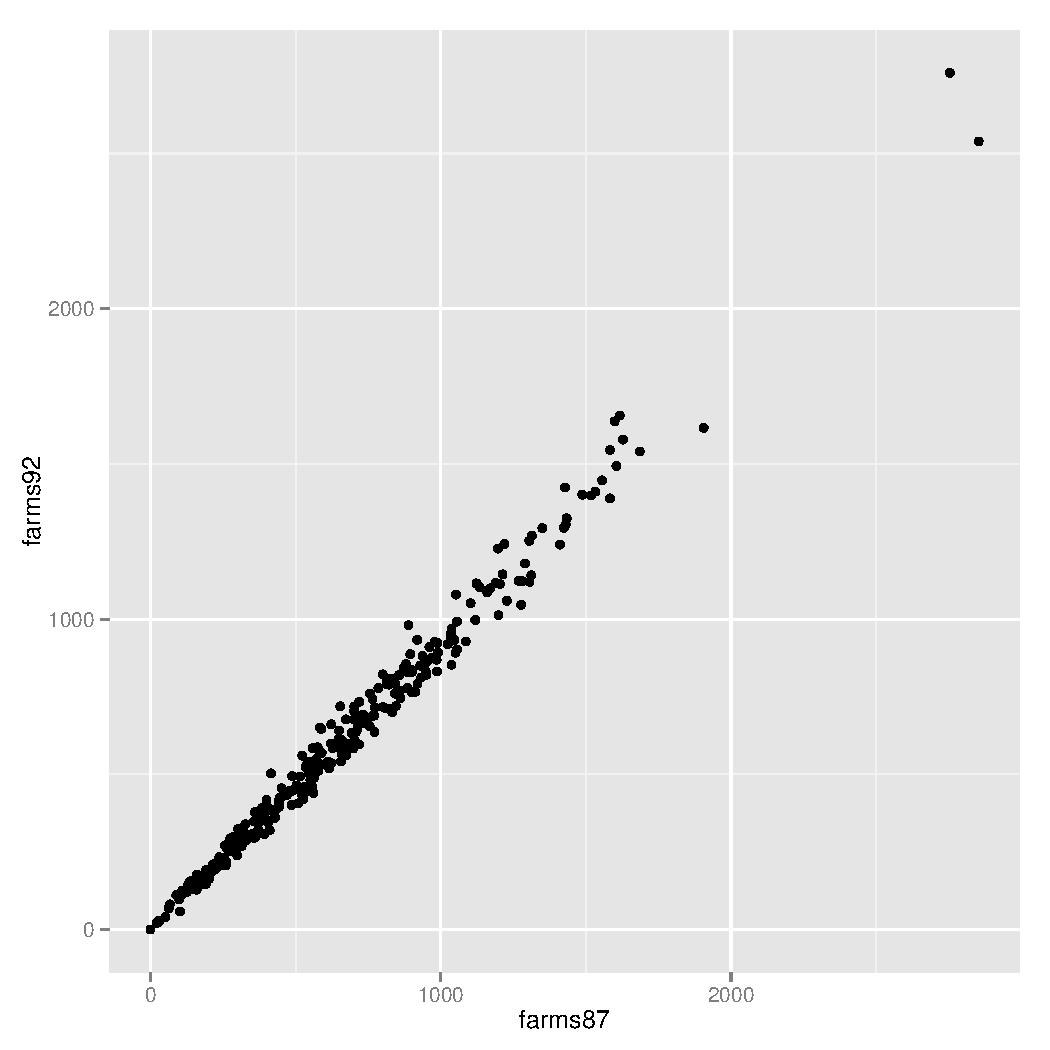
\includegraphics[width=.45\textwidth]{figure/unnamed-chunk-52} 

}


\end{knitrout}

\subsection*{Exercise 4.8 (b)}
\begin{knitrout}
\definecolor{shadecolor}{rgb}{0.969, 0.969, 0.969}\color{fgcolor}\begin{kframe}
\begin{alltt}
t.x <- 2087759
n <- 300
N <- 3078
(x.bar <- \hlfunctioncall{mean}(agsrs$farms87))
\end{alltt}
\begin{verbatim}
## [1] 647.7
\end{verbatim}
\begin{alltt}
(y.bar <- \hlfunctioncall{mean}(agsrs$farms92))
\end{alltt}
\begin{verbatim}
## [1] 599.1
\end{verbatim}
\begin{alltt}
(B.hat <- y.bar/x.bar)
\end{alltt}
\begin{verbatim}
## [1] 0.9248
\end{verbatim}
\begin{alltt}
t.hat.y.ratio <- B.hat * t.x
\hlfunctioncall{paste}(\hlstring{"ESTIMATOR OF POP MEAN VIA RATIO ===="}, t.hat.y.ratio)
\end{alltt}
\begin{verbatim}
## [1] "ESTIMATOR OF POP MEAN VIA RATIO ==== 1930836.49967065"
\end{verbatim}
\end{kframe}
\end{knitrout}

\subsection*{Exercise 4.8 (c)}
\begin{knitrout}
\definecolor{shadecolor}{rgb}{0.969, 0.969, 0.969}\color{fgcolor}\begin{kframe}
\begin{alltt}
(farms.coef <- \hlfunctioncall{with}(agsrs, \hlfunctioncall{simple.reg}(farms87, farms92)))
\end{alltt}
\begin{verbatim}
## [[1]]
## [1] -1.045
## 
## [[2]]
## [1] 0.9265
\end{verbatim}
\begin{alltt}
(y.bar.hat.reg <- farms.coef[[1]] + farms.coef[[2]] * t.x/N)
\end{alltt}
\begin{verbatim}
## [1] 627.4
\end{verbatim}
\begin{alltt}
(t.hat.y.regression <- y.bar.hat.reg * N)
\end{alltt}
\begin{verbatim}
## [1] 1930988
\end{verbatim}
\end{kframe}
\end{knitrout}


\end{document}
